\documentclass{article}
\usepackage{graphicx}
\usepackage[margin=1.5cm]{geometry}
\usepackage{amsmath}

\begin{document}

\title{Thursday Reading Assessment: ADC and DAC (Chapter 12 + Lab)}
\author{Prof. Jordan C. Hanson}

\maketitle

\begin{figure}[ht]
\centering
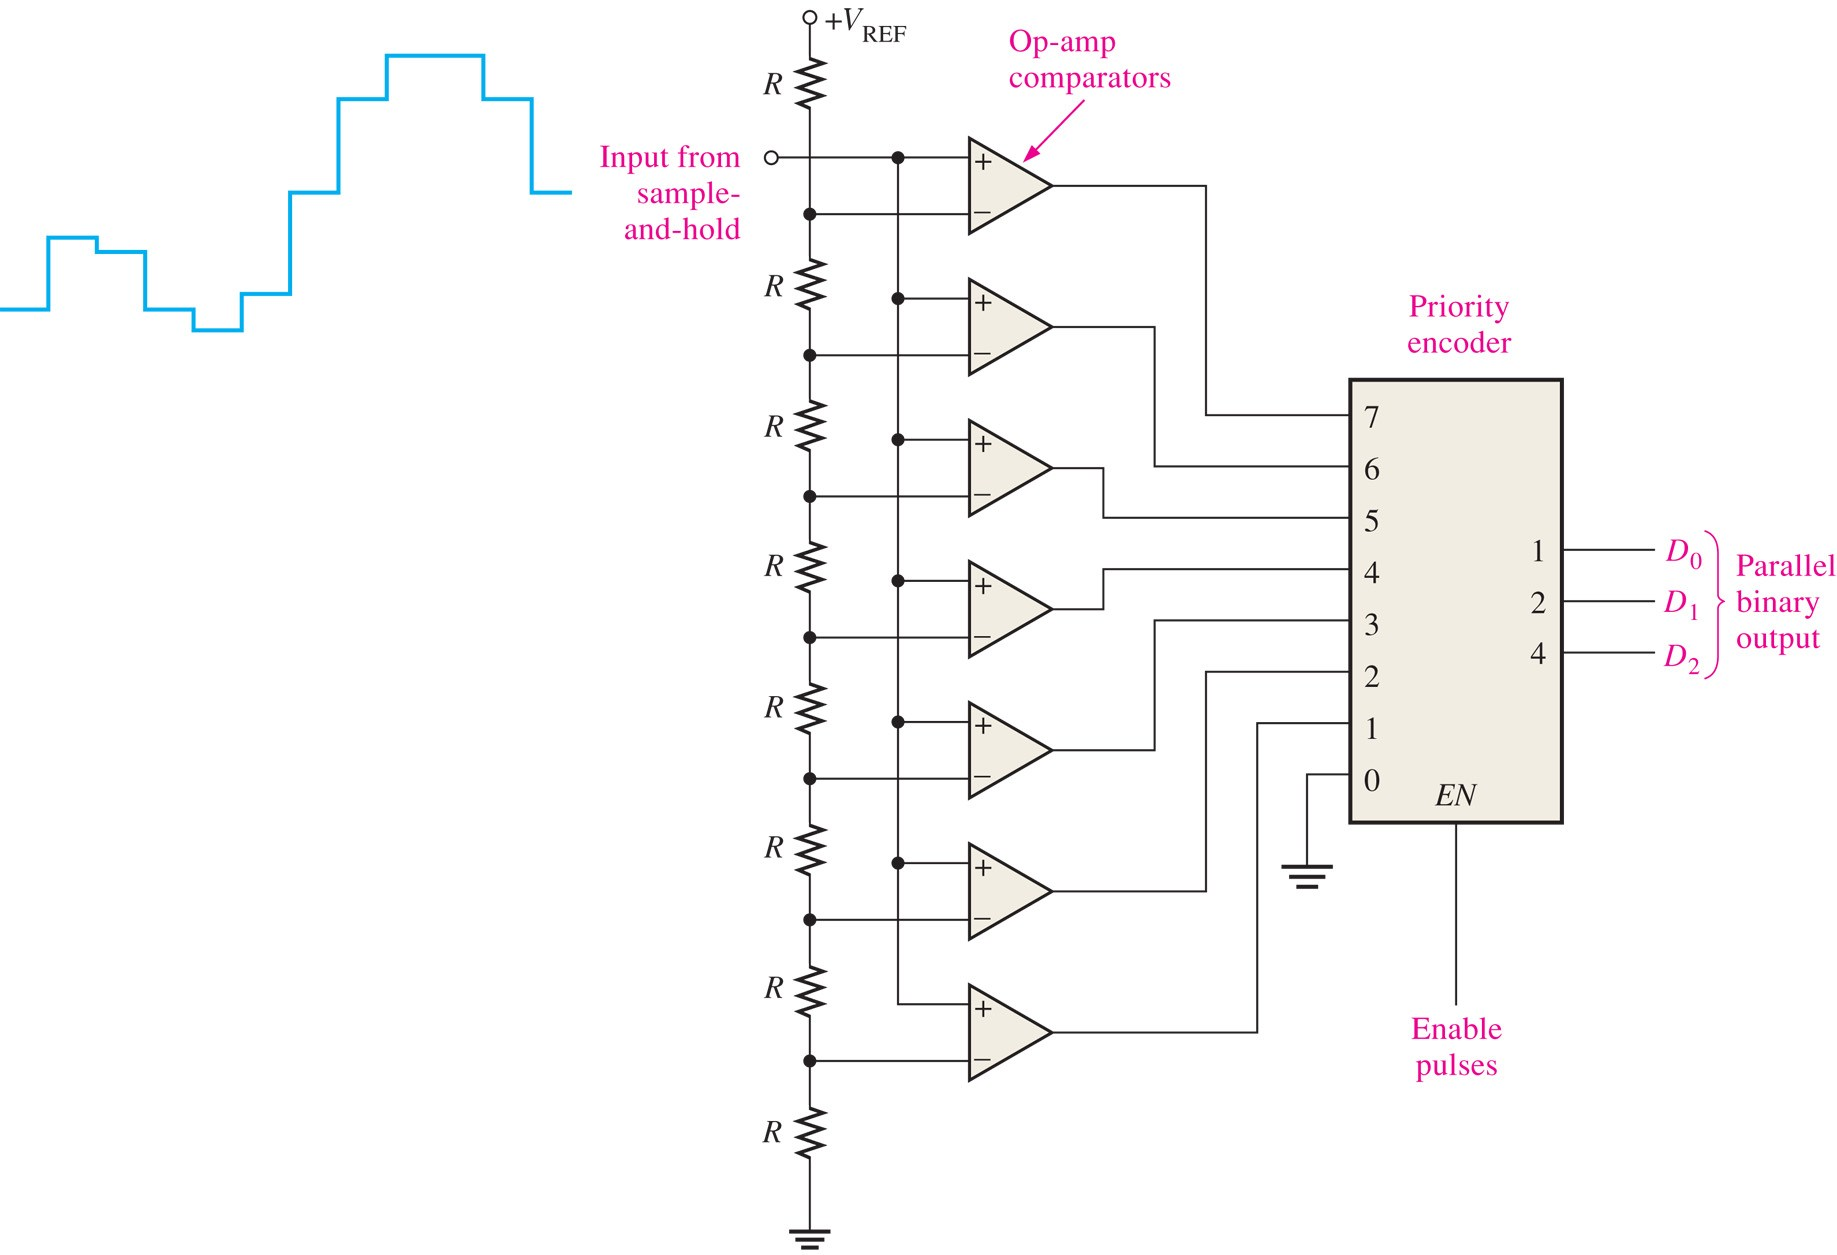
\includegraphics[width=0.35\textwidth,trim=6.0cm 0cm 0cm 0cm,clip=true]{figures/adc_6.jpg} \hspace{0.5cm}
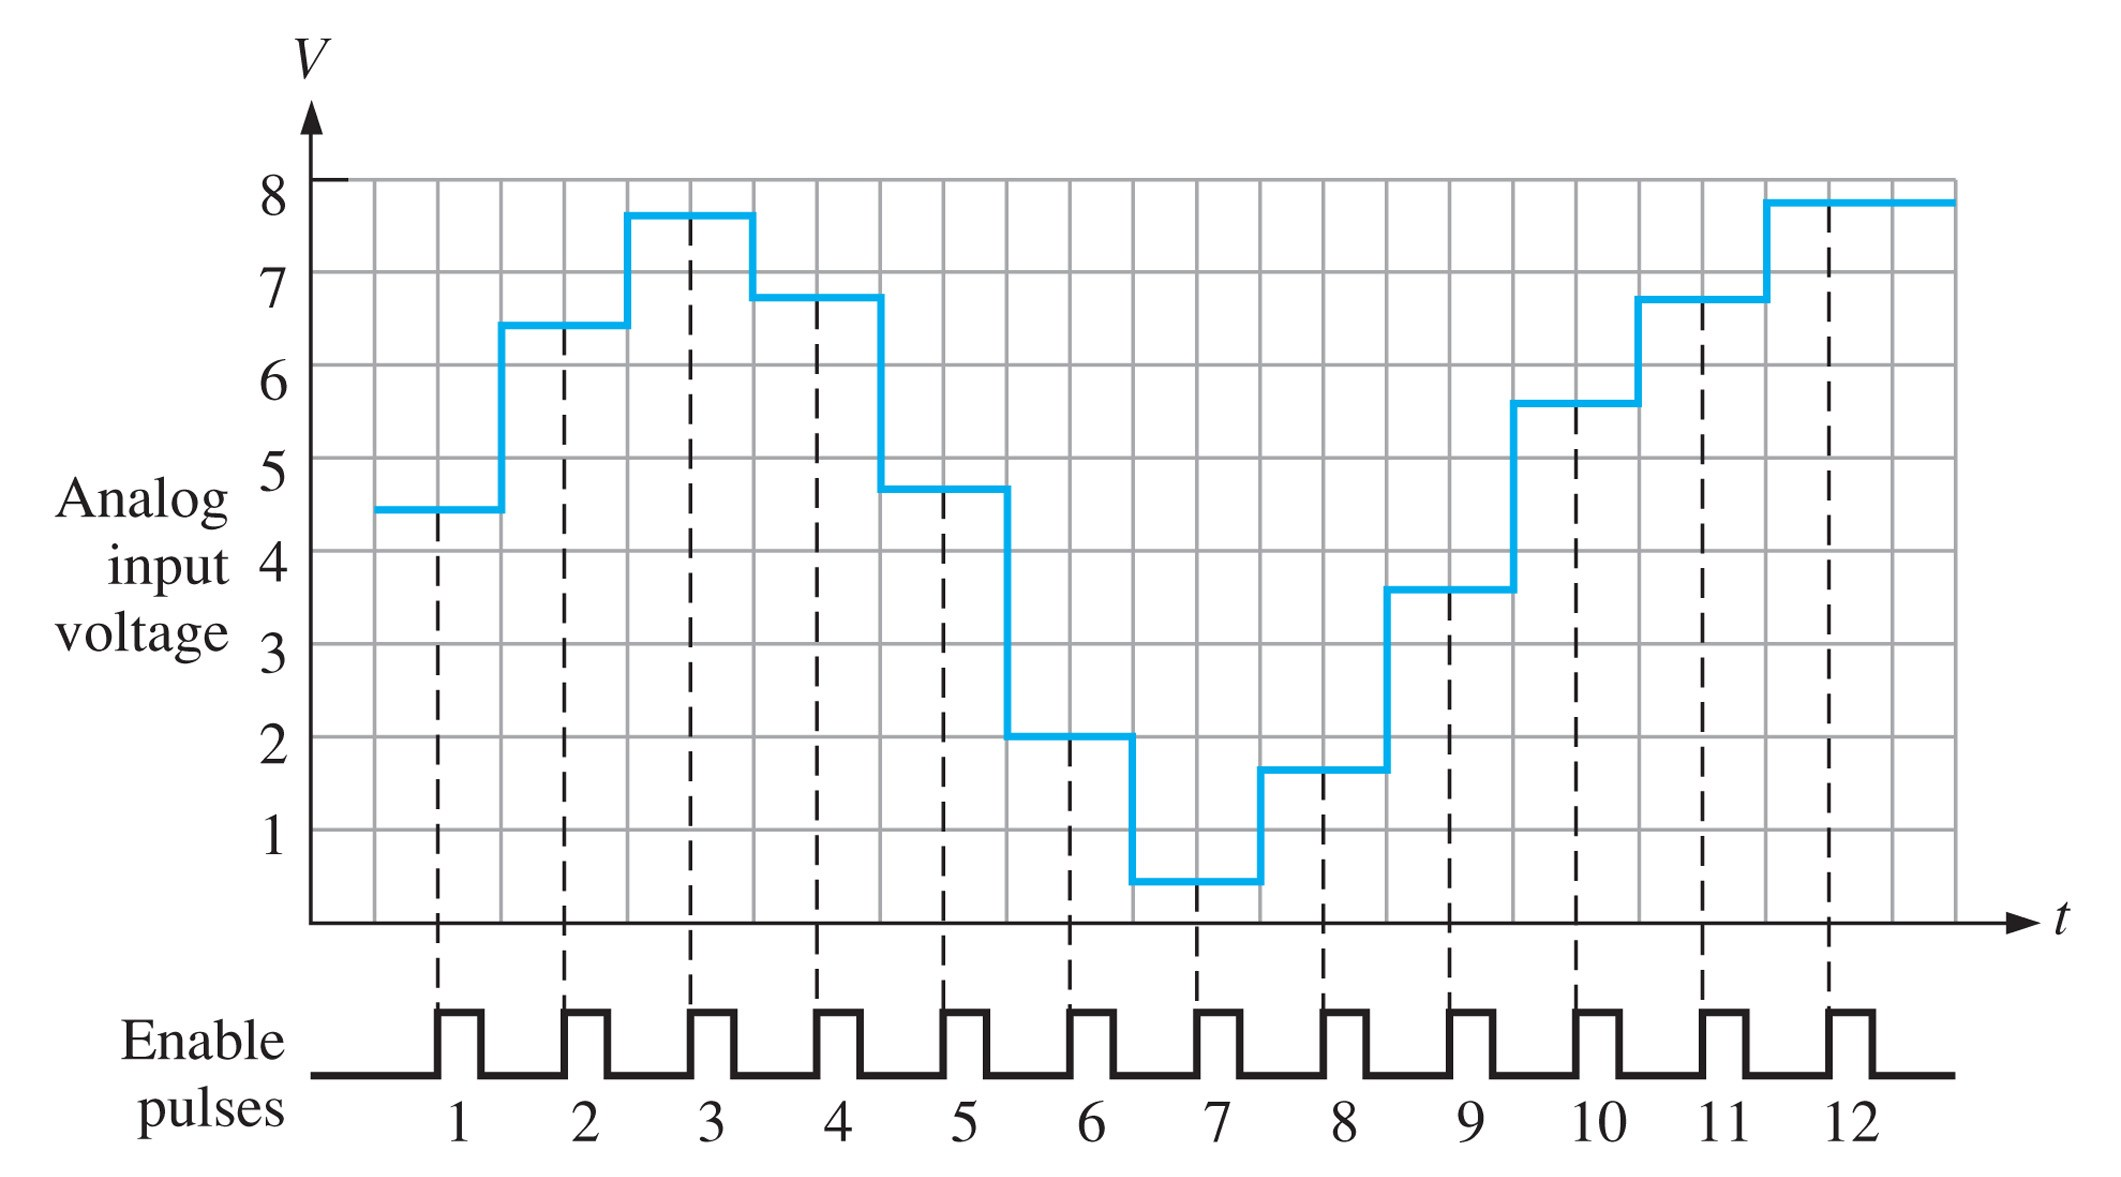
\includegraphics[width=0.55\textwidth]{figures/adc_7.jpg}
\caption{\label{fig:1} (Left) The 3-bit \textbf{Flash ADC}. (Right) The input to the 3-bit Flash ADC.}
\end{figure}

\section{Analog-to-Digital Conversion}

\begin{enumerate}
\item For the ADC in Fig. \ref{fig:1} (left), $V_{\rm ref} = +8$ Volts.  (a)  What is the voltage \textit{resolution}? (b) Determine the binary code output of the 3-bit flash ADC in Fig. \ref{fig:1} (left), given the input signal in Fig. \ref{fig:1} (right), given the encoder enable pulses shown. (c) If the enable pulse frequency in Fig. \ref{fig:1} (right) were halved, determine the binary numbers represented by the resulting digital output.  Is any information lost?
\end{enumerate}

\end{document}
